\documentclass{article}

\title{\sc\LARGE CSCA67 Tutorial, Week 1\\
{\Large Sept. 14th-18th, 2015}}
\date{}
\author{\sc Compiled by {\em G. Singh Cadieux}\\[1ex]
\sc Adapted from\\
A. Bretscher, \href{http://www.utsc.utoronto.ca/~bretscher/a67/lectures/w1.pdf}{\em CSCA67 Week 1 Lecture Notes},\\
\href{http://www.intmath.com/counting-probability/2-basic-principles-counting.php}{\em Interactive Mathematics: Basic Principles of Counting} \&\\
Lov\'{a}sz, et al. \textit{Discrete Mathematics: Elementary and Beyond.} Springer, 2003.}

\usepackage{fullpage}
\usepackage{amsmath,amssymb}
\usepackage{color}
\usepackage{multicol}
\usepackage{tikz}
\usepackage{hyperref}

\setlength{\parindent}{0pt}

\begin{document}
\maketitle

\section{\sc Review of week 1's lecture}
\subsection*{\em A Counting Problem}

Consider a \href{https://www.youtube.com/watch?v=xak-onyKwyA}{pizza commercial} that advertises\dots
\begin{itemize}
\item 2 pizzas
\item up to 5 toppings on each
\item 11 toppings to choose from
\end{itemize}

\subsubsection*{\sc Q: How many different combinations of 2 pizzas exist?}
\textsc{First,} how many combinations of up to 5 toppings exist for 1 pizza?
\begin{multline*}
\text{\bf\# of combinations of \textit{up to} 5 toppings}=\\\text{\# of combinations of no toppings }+
\shoveright{\text{ \# of combinations of 1 topping }+\ldots+}\\
\text{ \# of combinations of 4 toppings }+\text{ \# of combinations of 5 toppings}
\end{multline*}

\begin{itemize}
\item There is only 1 way to ``combine" no toppings.\\
$\Rightarrow\text{\bf\# of combinations of no toppings}=1$

\item There are 11 choices of toppings, meaning that there are 11 ways to ``combine" a single topping.\\
$\Rightarrow\text{\bf\# of combinations of 1 topping}=11$

\item There are 11 different ways to choose a single topping. Once the first topping has been chosen, there are 10 other topping choices. This means that there are $11\times 10$ ways to choose 2 toppings.\\[1ex]
\textit{However}, some of the combinations of 2 toppings are equivalent, since the order in which the toppings are selected does not matter.\\[1ex]
Eg., $\underbrace{\text{tomatoes}}_{\text{topping1}},\,\underbrace{\text{cheese}}_{\text{topping2}}\Leftrightarrow\underbrace{\text{cheese}}_{\text{topping1}},\,\underbrace{\text{tomatoes}}_{\text{topping2}}$\\[1em]
How many combinations are equivalent?\\[1ex]
Every combination of 2 toppings is equivalent to one other combination in which the order of the 2 toppings is reversed (see ex. above). This means that only \textit{half} of the $11\times 10$ ways are unique.\\[1ex]
$\Rightarrow\text{\bf\# of combinations of 2 toppings}=\dfrac{11\cdot 10}{2}$

\item There are 11 different ways to choose a single topping. Once the first topping has been chosen, there are 10 other topping choices. Once the second topping has been chosen, there are 9 other topping choices. This means that there are $11\times 10\times 9$ ways to choose 3 toppings.\\[1ex]
However, once again, some of the combinations are equivalent. How many?\\[1ex]
Suppose that we choose 3 toppings. In how many different orders can we choose these 3 toppings?\\
There are 3 different ways to choose the first topping. Then there are 2 ways to choose the second, and 1 way to choose the third.\\[1ex]
Eg., $\underbrace{\text{tomatoes}}_{\text{topping1}},\,\underbrace{\text{cheese}}_{\text{topping2}},\,\underbrace{\text{olives}}_{\text{topping3}}
\Leftrightarrow\underbrace{\text{tomatoes}}_{\text{topping1}},\,\underbrace{\text{olives}}_{\text{topping2}}\,\underbrace{\text{cheese}}_{\text{topping3}}
\Leftrightarrow\underbrace{\text{cheese}}_{\text{topping1}},\,\underbrace{\text{olives}}_{\text{topping2}}\,\underbrace{\text{tomatoes}}_{\text{topping3}}
\Leftrightarrow\ldots$\\[1em]
This means that there are $3\times 2\times 1$ different orderings of 3 toppings, and $3\times 2\times 1$ equivalent combinations of 3 toppings in different orders. So only $\frac{1}{3\cdot 2\cdot 1}$, or 1 out of 6, of the $11\times 10\times 9$ ways are unique.\\[1ex]
$\Rightarrow\text{\bf\# of combinations of 3 toppings}=\dfrac{11\cdot 10\cdot 9}{3\cdot 2\cdot 1}$

\item By extension of the reasoning above, there are $11\times 10\times 9\times 8$ ways to choose 4 toppings. But there are $4\times 3\times 2\times 1$ ways of ordering 4 chosen toppings, meaning that only $\frac{1}{4\cdot 3\cdot 2\cdot 1}$ of the $11\times 10\times 9\times 8$ ways are unique.\\[1ex]
$\Rightarrow\text{\bf\# of combinations of 4 toppings}=\dfrac{11\cdot 10\cdot 9\cdot 8}{4\cdot 3\cdot 2\cdot 1}$

\item Finally, by extension again,\\[1ex]
$\text{\bf\# of combinations of 5 toppings}=\dfrac{11\cdot 10\cdot 9\cdot 8\cdot 7}{5\cdot 4\cdot 3\cdot 2\cdot 1}$
\end{itemize}

\begin{align*}
\therefore\text{ \# of combinations of \textit{up to} 5 toppings}& =1+11+\dfrac{11\cdot 10}{2}+\dfrac{11\cdot 10\cdot 9}{3\cdot 2\cdot 1}+\dfrac{11\cdot 10\cdot 9\cdot 8}{4\cdot 3\cdot 2\cdot 1}+\dfrac{11\cdot 10\cdot 9\cdot 8\cdot 7}{5\cdot 4\cdot 3\cdot 2\cdot 1}\\
& =1+11+55+165+330+462\\
& =1024
\end{align*}

\textsc{Second,} how many combinations of 2 pizzas exist?
\begin{multline*}
\text{\bf\# of combinations of 2 pizzas}=\\
\text{\# of combinations of 2 different pizzas }+\text{ \# of combinations of 2 of the same pizza}
\end{multline*}

\begin{itemize}
\item There are 1024 possible unique pizzas from which to choose a single pizza. Once the first pizza has been chosen, there are 1023 different choices for the second pizza.\\[1ex]
However, once again, the order in which the 2 pizzas are selected does not matter. So, as in the case of selecting 2 toppings for a pizza, every combination of 2 different pizzas \{pizza1, pizza2\} is equivalent to another combination \{pizza2, pizza1\}, in which the order is reversed.\\[1ex]
$\Rightarrow\text{\bf\# of combinations of 2 different pizzas}=\dfrac{1024\cdot 1023}{2}$
\item There are 1024 possible unique pizzas, meaning that there are 1024 ways to combine 2 of the same pizza.\\[1ex]
$\Rightarrow\text{\bf\# of combinations of 2 of the same pizza}=1024$
\end{itemize}

\begin{align*}
\therefore\text{ \sc\# of combinations of 2 pizzas}& =\dfrac{1024\cdot 1023}{2}+1024\\
& =523\;776+1024\\
& =524\;800
\end{align*}

\textsc{N.B. There are} several possible, equally valid ways to arrive at this answer, including different methods that may have been demonstrated in lecture, and different methods which we will see in the upcoming weeks.

\section{\sc Counting problems}

\subsection*{Q: {\em In how many ways can a number be chosen from 1 to 22 such that}}
\subsubsection*{a) {\em it is a multiple of 3 or 8?}}
Multiples of 3 from 1 to 22: {\color{red}3, 6, 9, 12, 15, 18, 21}\\[1ex]
Multiples of 8 from 1 to 22: {\color{blue}8, 16}\\[1em]
Multiples of 3 \textit{or} 8 from 1 to 22: {\color{red}3, 6,} {\color{blue}8,} {\color{red}9, 12, 15,} {\color{blue}16,} {\color{red}18, 21}\\[1ex]
$\therefore$ There are 9 multiples of 3 or 8 from which to choose.

\subsubsection*{b) {\em it is a multiple of 2 or 3?}}
Multiples of 2 from 1 to 22: {\color{red}2, 4, 6, 8, 10, 12, 14, 16, 18, 20, 22}\\[1ex]
Multiples of 3 from 1 to 22: {\color{blue}3, 6, 9, 12, 15, 18, 21}\\[1em]
Notice that some of these multiples are not unique: for instance, 6 is a multiple of both 2 \textit{and} 3. We only consider these numbers once.\\[1ex]
Multiples of 2 \textit{or} 3 from 1 to 22: {\color{red}2,} {\color{blue}3,} {\color{red}4,} 6, {\color{red}8,} {\color{blue}9,} {\color{red}10,} 12, {\color{red}14,} {\color{blue}15,} {\color{red}16,} 18, {\color{red}20,} {\color{blue}21,} {\color{red}22}\\[1ex]
$\therefore$ There are 15 multiples of 2 or 3 from which to choose.\\[1em]
We can also represent this as a \textit{Venn diagram}:\\[1ex]
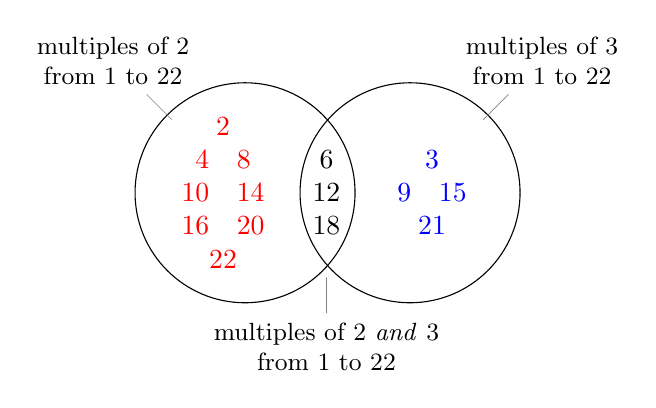
\begin{tikzpicture}[scale=1.1]
\draw (0,0) circle[radius=0.5in];
\draw (0.75in,0) circle[radius=0.5in];
\node[align=center,font={\small},pin=below right:{}] at (-0.6in,0.6in) {multiples of 2\\ from 1 to 22};
\node[align=center,font={\small},pin=below left:{}] at (1.35in,0.6in) {multiples of 3\\ from 1 to 22};
\node[align=center,font={\small},pin=above:{}] at (0.37in,-0.7in) {multiples of 2 \textit{and} 3\\ from 1 to 22};
\node[align=center,color=red] at (-.1in,0) {2\\4\quad 8\\10\quad 14\\16\quad 20\\22};
\node[align=center] at (.37in,0) {6\\12\\18};
\node[align=center,color=blue] at (.85in,0) {3\\9\quad 15\\21};
\end{tikzpicture}

\subsection*{{\normalsize Suppose you have 2 t-shirts and 4 pairs of jeans.}\\
Q: {\em How many combinations of 1 t-shirt and 1 pair of jeans can you make?}}
Let's enumerate all the combinations:\\[1ex]
\begin{tabular}{lcclc}
(1)&\{T1, J1\}&&(5)&\{T2, J1\}\\
(2)&\{T1, J2\}&&(6)&\{T2, J2\}\\
(3)&\{T1, J3\}&&(7)&\{T2, J3\}\\
(4)&\{T1, J4\}&&(8)&\{T2, J4\}
\end{tabular}\\[1em]
Alternatively, the combinations can be depicted with trees:\\[1ex]
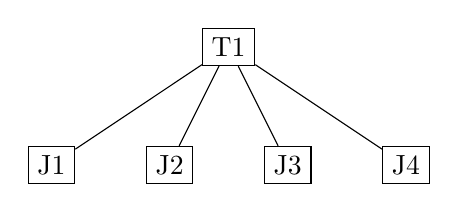
\begin{tikzpicture}
\node[rectangle,draw]{T1}
child{node[rectangle,draw]{J1}}
child{node[rectangle,draw]{J2}}
child{node[rectangle,draw]{J3}}
child{node[rectangle,draw]{J4}};
\end{tikzpicture}
\quad
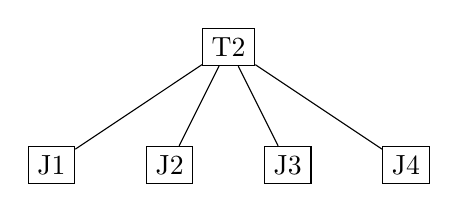
\begin{tikzpicture}
\node[rectangle,draw]{T2}
child{node[rectangle,draw]{J1}}
child{node[rectangle,draw]{J2}}
child{node[rectangle,draw]{J3}}
child{node[rectangle,draw]{J4}};
\end{tikzpicture}\\[1em]
We can see that there are 8 combinations in total.\\[1ex]
If we first choose a t-shirt, there are 2 ways that we can do so. Then, there are 4 ways to choose a pair of jeans.
$2\times 4$ gives us the total number of combinations.\\[1em]
\textsc{In general,} there are $n\times m$ ways to combine 1 object from a set of $n$ objects with 1 object from another set of $m$ objects.

\subsection*{{\normalsize The life insurance policies of an insurance company are classified by:\\[1ex]
\begin{tabular}{p{0.3\textwidth}p{0.3\textwidth}p{0.3\textwidth}}
(i) age of the insured
	\begin{itemize}
	\item under 25 years
	\item 25-50 years
	\item over 50 years
	\end{itemize}
&(ii) sex
	\begin{itemize}
	\item male
	\item female
	\end{itemize}
&(iii) marital status
	\begin{itemize}
	\item single
	\item married
	\end{itemize}
\end{tabular}\\
An example of a policy classification is \{25-50 years, male, single\}.}\\
Q: {\em What is the total number of classifications?}}
Using the multiplication principle from above, we say that there are
\begin{equation*}
3\text{ ages}\times 2\text{ sexes}\times 2\text{ marital statuses}=12\text{ total classifications}
\end{equation*}

\subsection*{{\normalsize On \href{http://mono-1.com/monoface/main.html}{mono-1.com/monoface}, we can combine different people's facial features to form a composite face. We are told that there are 759 375 possible composite faces.}\\
Q: {\em How did they calculate the total number of faces?}}
There are 5 features that we can change: head \& shoulders, right eye, left eye, nose, mouth.\\
For each of these features, there are 15 possible variations.\\[1ex]
Using the multiplication principle, we determine that there are
\begin{equation*}
[15\text{ head \& shoulders}]\times[15\text{ right eye}]\times\ldots\times[15\text{ mouth}]=15^5=759\,375\text{ combinations of features}
\end{equation*}

\subsubsection*{Q: {\em If they let us change the chin as well, how many possible combinations would there be?}}
We would then have 6 features to change, and 15 variations of each of these features.\\
As above, we say that there would be
\begin{equation*}
[15\text{ head \& shoulders}]\times\ldots\times[15\text{ mouth}]\times[15\text{ chin}]=15^6=11\,390\,625\text{ combinations of features}
\end{equation*}

\section{\sc Additional practice problems}

7 people are going to a party: Alice, Bob, Carl, Diane, Eve, Frank, and George.\\
When they have all arrived, everyone shakes hands.\\
{\bf Q: How many handshakes were there altogether?}\\[1em]
They then go to the table to eat, but they can't agree on the seating arrangement.\\
{\bf Q: How many possibilities are there if Alice always stays at the head (since it is her birthday)?}\\[1ex]
{\bf Q: How many possibilities are there if Alice can sit anywhere?}\\[1em]
They decide to play bridge after dinner. When the cards have been dealt, Carl says that he thinks he got the same hand as last time.\\
{\bf Q: What is the likelihood that he is right?}\\[1em]
Finally, they decide to play chess. Alice just wants to watch, and sets up 3 boards.\\
{\bf Q: How many different ways can they be matched?}

\end{document}